\documentclass[twocolumn]{article}
\usepackage{graphicx}
\usepackage{amsmath,amsthm,amssymb,amsfonts, enumitem, fancyhdr, color, comment, graphicx, environ, lastpage}
\pagestyle{fancy}
\setlength{\headheight}{65pt}

\lhead{Ruida Zhou, Hongqian Xia\\ Angelo De Nadai, Joel Dettinger}  %replace with your name
\rhead{WDPS Fall 24\\Group 28} %replace XYZ with the homework course number, semester (e.g. ``Spring 2019"), and assignment number.
\fancyfoot[C]{page \thepage/\pageref{LastPage}} % Centered footer with page numbers


\begin{document}
\section{Introduction}
The report is for the WDPS project submitted by Group 28. In this project, we implemented a post-processor that 1) links Wikipedia entities to LLM responses to user questions, 2) extracts Y/N or entity answers from the responses, and 3) fact checks the answers. For each of the aforementioned three key tasks, we don't use any one-library-does-it-all solution but rather we break them into subtasks as shown below in Figure 1.1 and leverage carefully picked libraries and tools.\\
\begin{figure}[h!]
    \centering
    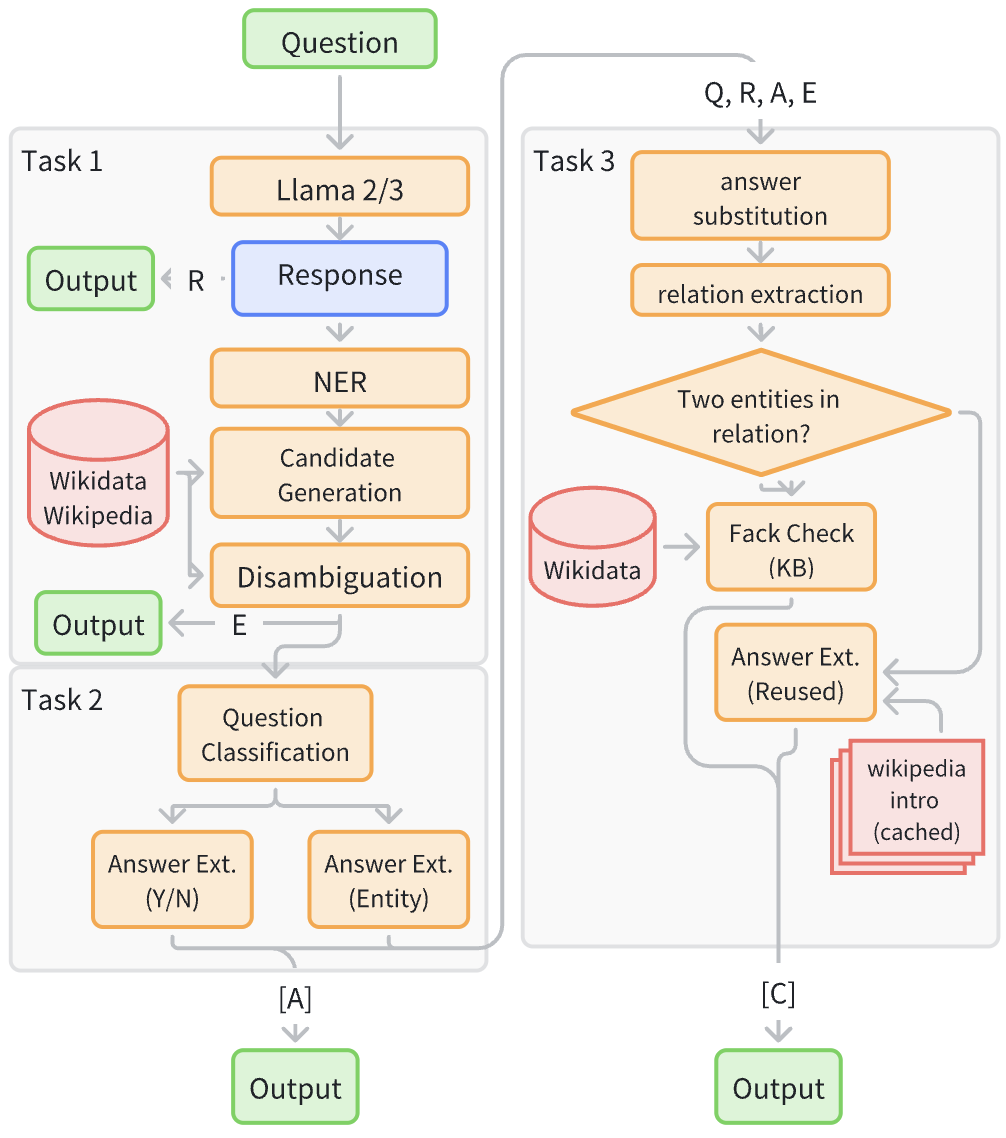
\includegraphics[width=0.5\textwidth]{./intro.png}
    \caption{Overall Structure}
\end{figure}\\
Tested with multiple cases on Llama 2 and 3, the postprocessor extracts almost all named entities correctly, links to the correct Wikipedia page with high precision and recall, and always extracts Y/N or entity answers correctly. The fact checker works well for 3/5 of the example questions and is capable of checking all additional test cases that we compiled.\\
The postprocessor is implemented with scalability in mind and applies simple but effective heuristics to reduce requests issued to Wikipedia.
\section{Design}
\subsection{Entity linking}
We use SOTA ML models for NER. Candidate entities are drawn from Wikidata. Exact matching and embedding are used for disambiguation. Coherence between entities is also exploited for disambiguation.
\vskip 0.95em \noindent 
Named entities are extracted using \textit{SpaCy}. An edge case is that it recognizes ``Pulp Fiction is Quentin Tarantino'' as one named entity. \textit{bert-base-NER} is used for a second check on the extracted mentions of entities to fix the case. The context is also saved for disambiguation.
\vskip 0.95em \noindent 
The mentions to the entities are then searched on Wikidata to find top ten candidates ranked by the number of links to the entity (i.e. popularity). Each mention is further exact matched to see if it is a substring of any of the candidates. If such exact match is found, candidates are reduced to exact matches in order to request Wikipedia less.
\vskip 0.95em \noindent 
For candidates filtered with exact match, the first paragraph of the Wikipedia page of each candidate is fetched. Embeddings are computed by \textit{distilbert-base-uncased} to find the closest candidate to the mention. For each of the candidates, the embedding of the first paragraph of the corresponding Wikipedia entry is computed. Then the cosine similarity between the embedding of the mention and the embedding of the candidate is computed; the candidate with the highest similarity is chosen as the correct entity. 
\vskip 0.95em \noindent
In cases where the embeddings don't give a clear answer, these mentions are saved and queried on Wikidata again, but this time ranked with the number of links to the entities that are already confirmed. A candidate with more links to other confirmed entities in the context is likely to be a better option than candidates that are not related to any other confirmed entities. The approach is highly effective. For example, in the context of ancient Roman mythology, when linking the mention ``Rome'', the city of Rome has more existing links to confirmed entities like ``Mars'' than the TV series Rome does. Indeed, the city of Rome is the correct choice.
\vskip 0.95em \noindent
We design the part with scalability in mind and first tried locally deployed yago and go to Wikidata when yago fails. However, the mini version of yago has too few entities and querying again to exploit links between entities would be hard to implement with both yago and wikidata being used at the same time. We carefully limit results to the top 10 in SPARQL queries, and filter the results with exact match and embedding to reduce queries to Wikipedia and, on rare circumstances, Wikidata (to exploit links).
\subsection{Answer extraction}
First, we use the \textit{``shahrukhx01/question-vs-statement-classifier''} model to tell statements (``Sky is blue'') from questions. It is assumed that statements expect Y/N answers. Then the \textit{``PrimeQA/tydiqa-boolean-question-classifier''} model is used to tell whether the question expects a Y/N answer or an entity. Two deberta models are used to extract answers, namely \textit{``nfliu/deberta-v3-large\_boolq''} and \textit{``deepset/deberta-v3-base-squad2''}.
\subsection{Fact checking}
Two approaches are implemented for fact checking. The relation based approach is tried first before reusing the answer extraction module again.
\vskip 0.95em \noindent
The relation based approach extracts relation of $<$entity, relation, entity$>$ using Stanford coreNLP. Then, it searches for such a tuple in Wikidata and then compares the description of candidate relations with the extracted relation while reusing the embedding distance computed by the entity linking module. A close enough match implies correctness, otherwise the response is consider made up and incorrect. To enable the extraction of relations on questions expecting an entity, the concluded answer is substituted back to the question, guided by recognizing WH-words with \textit{nltk}.
\vskip 0.95em \noindent
Sometimes there is only one entity in the extracted relation (``India is the most populous country''). In this case, an entity is concluded from the response and the yes/no concluder is applied to (Question, first paragraph of the Wikipedia page of the entity) to conclude a Y/N answer. If the fact checking Y/N answer agrees with the previously extracted Y/N answer, it is considered correct.
\section{Conclusion}
We found that the pragmatic approach combining the symbolic KB and latent models is highly effective. In the entity linking part, the exact matching significantly improves the precision of the entity linking. The embedding based model is good at telling the difference between the fruit Apple and the company. However, it chooses Mac for a mention of ``Apple'' in the context of news related to technology over the company and the exact match heuristic eliminates unrelated candidates which have close embeddings to the mention.
\vskip 0.95em \noindent
In fact checking we also complement the symbolic approach (relation based) with latent models. If a tuple with two entities can be extracted, the success rate is high. However, for cases with only one entity, the fact checker doesn't work and the Y/N concluder gives a good answer for cases like ``India/China is the most populous country'' by looking at Wikipedia's first paragraphs. Though the fact checker using the latent model is more versatile, it is not a panacea; it fails to tell if Apple has the most revenue with Amazon's wiki intro paragraph. This is because the entity concluder considers Amazon the answer entity to whether Apple is the company with the most revenue.
\vskip 0.95em \noindent
Although latent models, especially LLMs, are on the trend, the pragmatic approach of combining latent models with the aid of the symbolic KB provides a versatile yet highly accurate solution to the postprocessing tasks discussed in this report.

\end{document}​​​​​​​​​​​​​​​